\documentclass{beamer}

%\begin{columns}[T]
%	\begin{column}{.5\textwidth}
%	\end{column}
%	\begin{column}{.5\textwidth}
%	\end{column}
%\end{columns}


\mode<presentation>
{
  \usetheme{Warsaw} % default or try Darmstadt, Madrid, Warsaw, ...
  \usecolortheme{default} % or try albatross, beaver, crane, ...
  \usefonttheme{default}  % or try serif, structurebold, ...
  \setbeamertemplate{navigation symbols}{}
  \setbeamertemplate{caption}[numbered]
} 

% ---------------------------------------------------------------------------
% PACKAGES
% ---------------------------------------------------------------------------
\usepackage{microtype}
\usepackage{cleveref} 
\usepackage[T1]{fontenc} % Use EC fonts
\usepackage{lmodern}
\usepackage[utf8]{inputenc}	% Encoding
\usepackage{csquotes} % To manage quotes
\usepackage[english]{babel} % Language selection
\usepackage{graphicx}
\usepackage{url}

\newcommand<>{\credit}[1]{\par\hfill \tiny \itshape \href{#1}{Source}}

\AtBeginSubsection[]
{
	\begin{frame}<beamer>
		\frametitle{Plan}
		\tableofcontents[currentsubsection]
	\end{frame}
}

% ---------------------------------------------------------------------------
% REFERENCING PACKAGE
% ---------------------------------------------------------------------------
\usepackage[backend=biber, citestyle=authoryear,doi=true,url=true]{biblatex}
\begin{filecontents}{references.bib}
	% @book{anderson,
	%	author = {Anderson, John D.},
	%	title = {{Fundamentals of Aerodynamics}},
	%	Publisher = {McGraw-Hill},
	%	year = {2011},
	%	edition = 5,
	%}
	@online{lumped,
		title = {Introduction and Lumped Circuit Abstraction},
		url = {https://6002x.mitx.mit.edu/static/handouts/6002-L1-oei12-gaps.pdf},
		urldate = {2017-01-01},
		author = {MIT},
		organization = {MIT},
	}
	@online{differentiation,
	title = {Sketching a Gradient Function},
	url = {http://maths.nayland.school.nz},
	urldate = {2017-01-01},
	author = {{Nayland College}}
	}
@report{intuition,
	author = {Erik Dane and  Michael Pratt},
	title = {Exploring intuition and its role in managerial decision making},
	institution = {University of Illinois at Urbana-Champaign},
	date = {2007},
}
@report{design,
	author = {Theo Humphries},
	title = {Considering intuition in the context of design, and of psychology},
	institution = {Cardiff Metropolitan University},
	date = {2012},
}
@report{berger,
	author = {Guy Berger},
	title = {Millennials Job-Hop More Than Previous Generations, \& They Aren't Slowing Down},
	institution = {LinkedIn},
	url = {https://www.linkedin.com/pulse/millennials-job-hop-more-than-previous-generations-guy-berger-ph-d-},
	date = {2016},
}
@book{gert,
	author = {Gert Gigerenzer},
	title = {Gut feelings},
	date = {2007},
}
\end{filecontents}
\addbibresource{references.bib}

\title[Importance of Intuition]{Importance of Intuition in Engineering}
\author{Vipin Ajayakumar}
\institute{Rolls-Royce}
\date{}

\begin{document}
\begin{frame}
  \titlepage
\end{frame}
\begin{frame}{Contents}
	\tableofcontents
\end{frame}

%=====================================================================
\section{Introduction}
%--------------------------------------------------------------------------------------------
\begin{frame}{About me}
	\begin{columns}[T]
		\begin{column}{.5\textwidth}
			\begin{itemize}[<+->]
				\item Aeroacoustics Engineer
				\item Data analysis and visualisation
			\end{itemize}
		\end{column}
		\begin{column}{.5\textwidth}
			\begin{figure}
				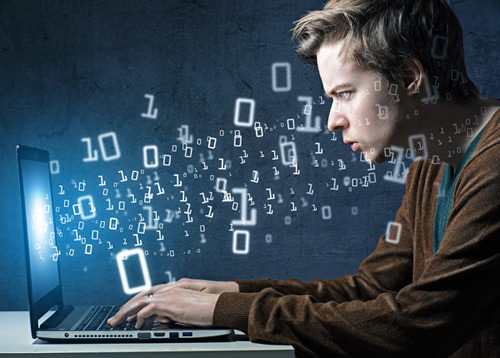
\includegraphics[width=\linewidth,height=\textheight,keepaspectratio]{images/programmer.jpg}
				\credit{http://media02.hongkiat.com/programming-myth/programmer.jpg}
			\end{figure}
		\end{column}
	\end{columns}
\end{frame}
\begin{frame}{Some of us are dependent on intuition!}
	\begin{figure}
		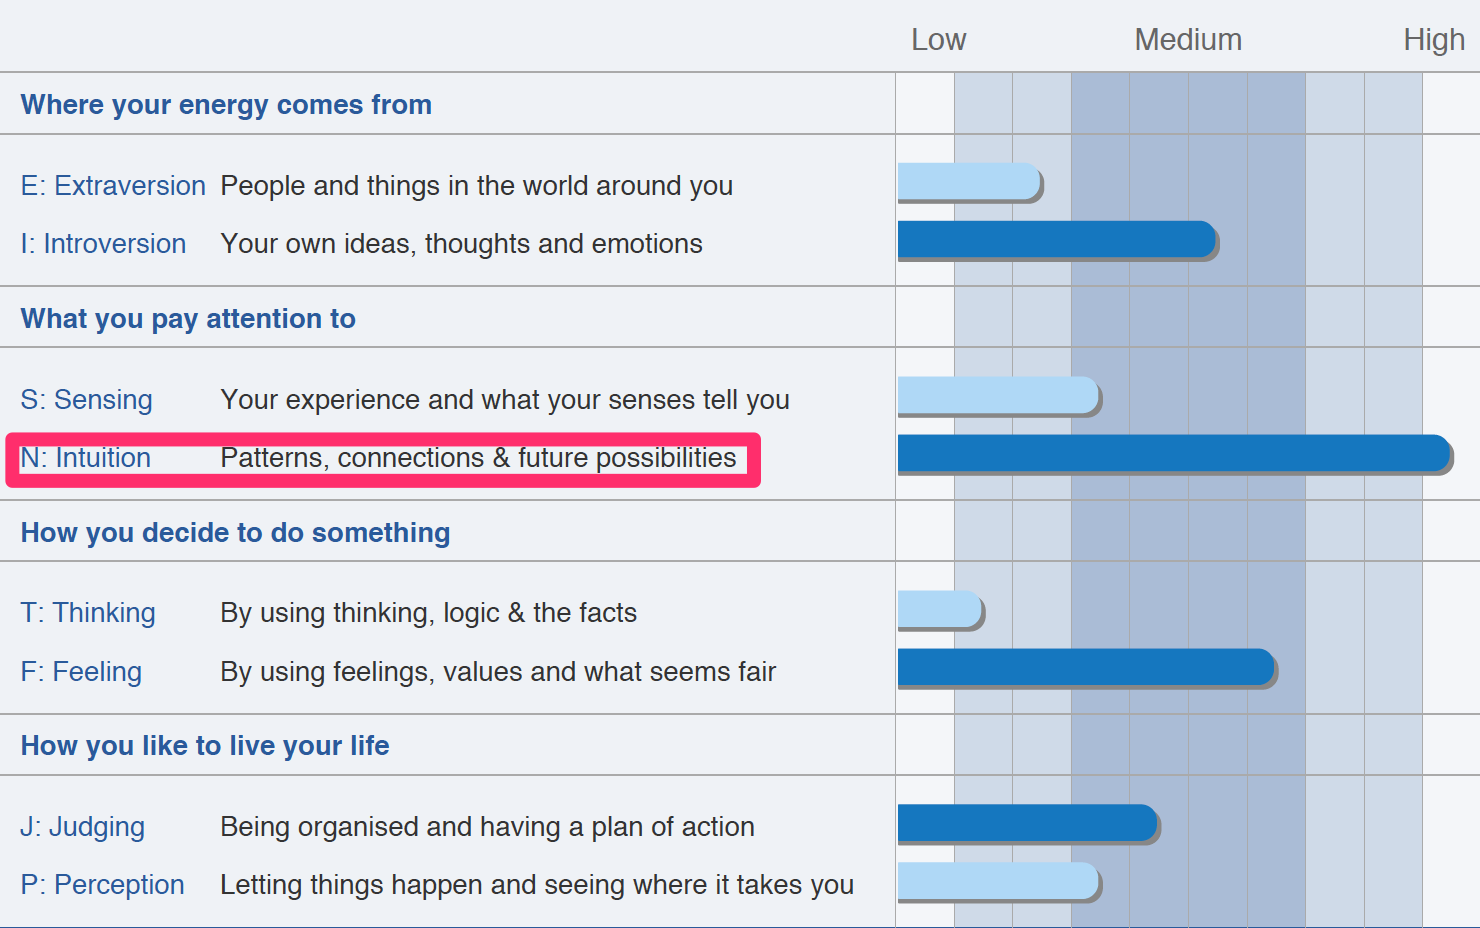
\includegraphics[width=\linewidth,height=0.7\textheight,keepaspectratio]{images/myprofile.png}
	\end{figure}
\end{frame}
\begin{frame}{Context}
%				\item Our work gets more and more complex day by day
%				\item Today, we don't have to wait for results thanks to technology
%				\item Is it worth setting aside time to master our subject, or should we just get on with the job?
			\begin{figure}
				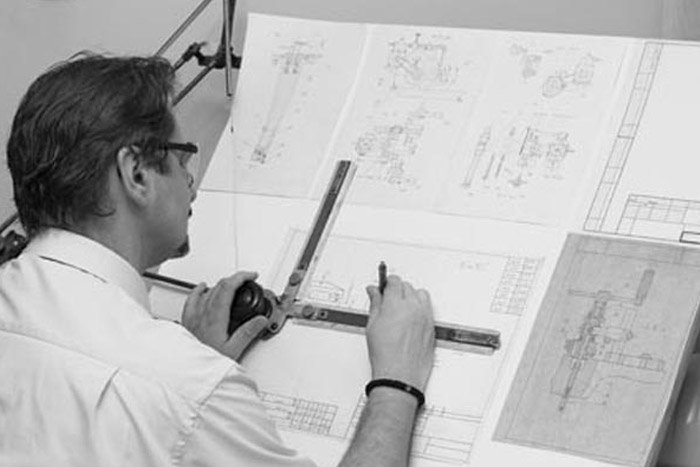
\includegraphics[width=\linewidth,height=0.7\textheight,keepaspectratio]{images/drawing.jpg}
				\caption{In the past, the slow pace of work forced us to think}
				\credit{https://sourceable.net/wp-content/uploads/2014/01/engineer-on-drawing-board.jpg}
			\end{figure}
\end{frame}
%=====================================================================
\section{The importance of intuition}
%--------------------------------------------------------------------------------------------
\subsection{What is intuition?}
%--------------------------------------------------------------------------------------------
\begin{frame}{Intuition}
	\begin{definition}
		The Oxford Dictionary defines \alert{intuitive}  as using or based on what one feels to be true even without conscious reasoning.
	\end{definition}
\end{frame}
\begin{frame}{Example}
	\begin{figure}
		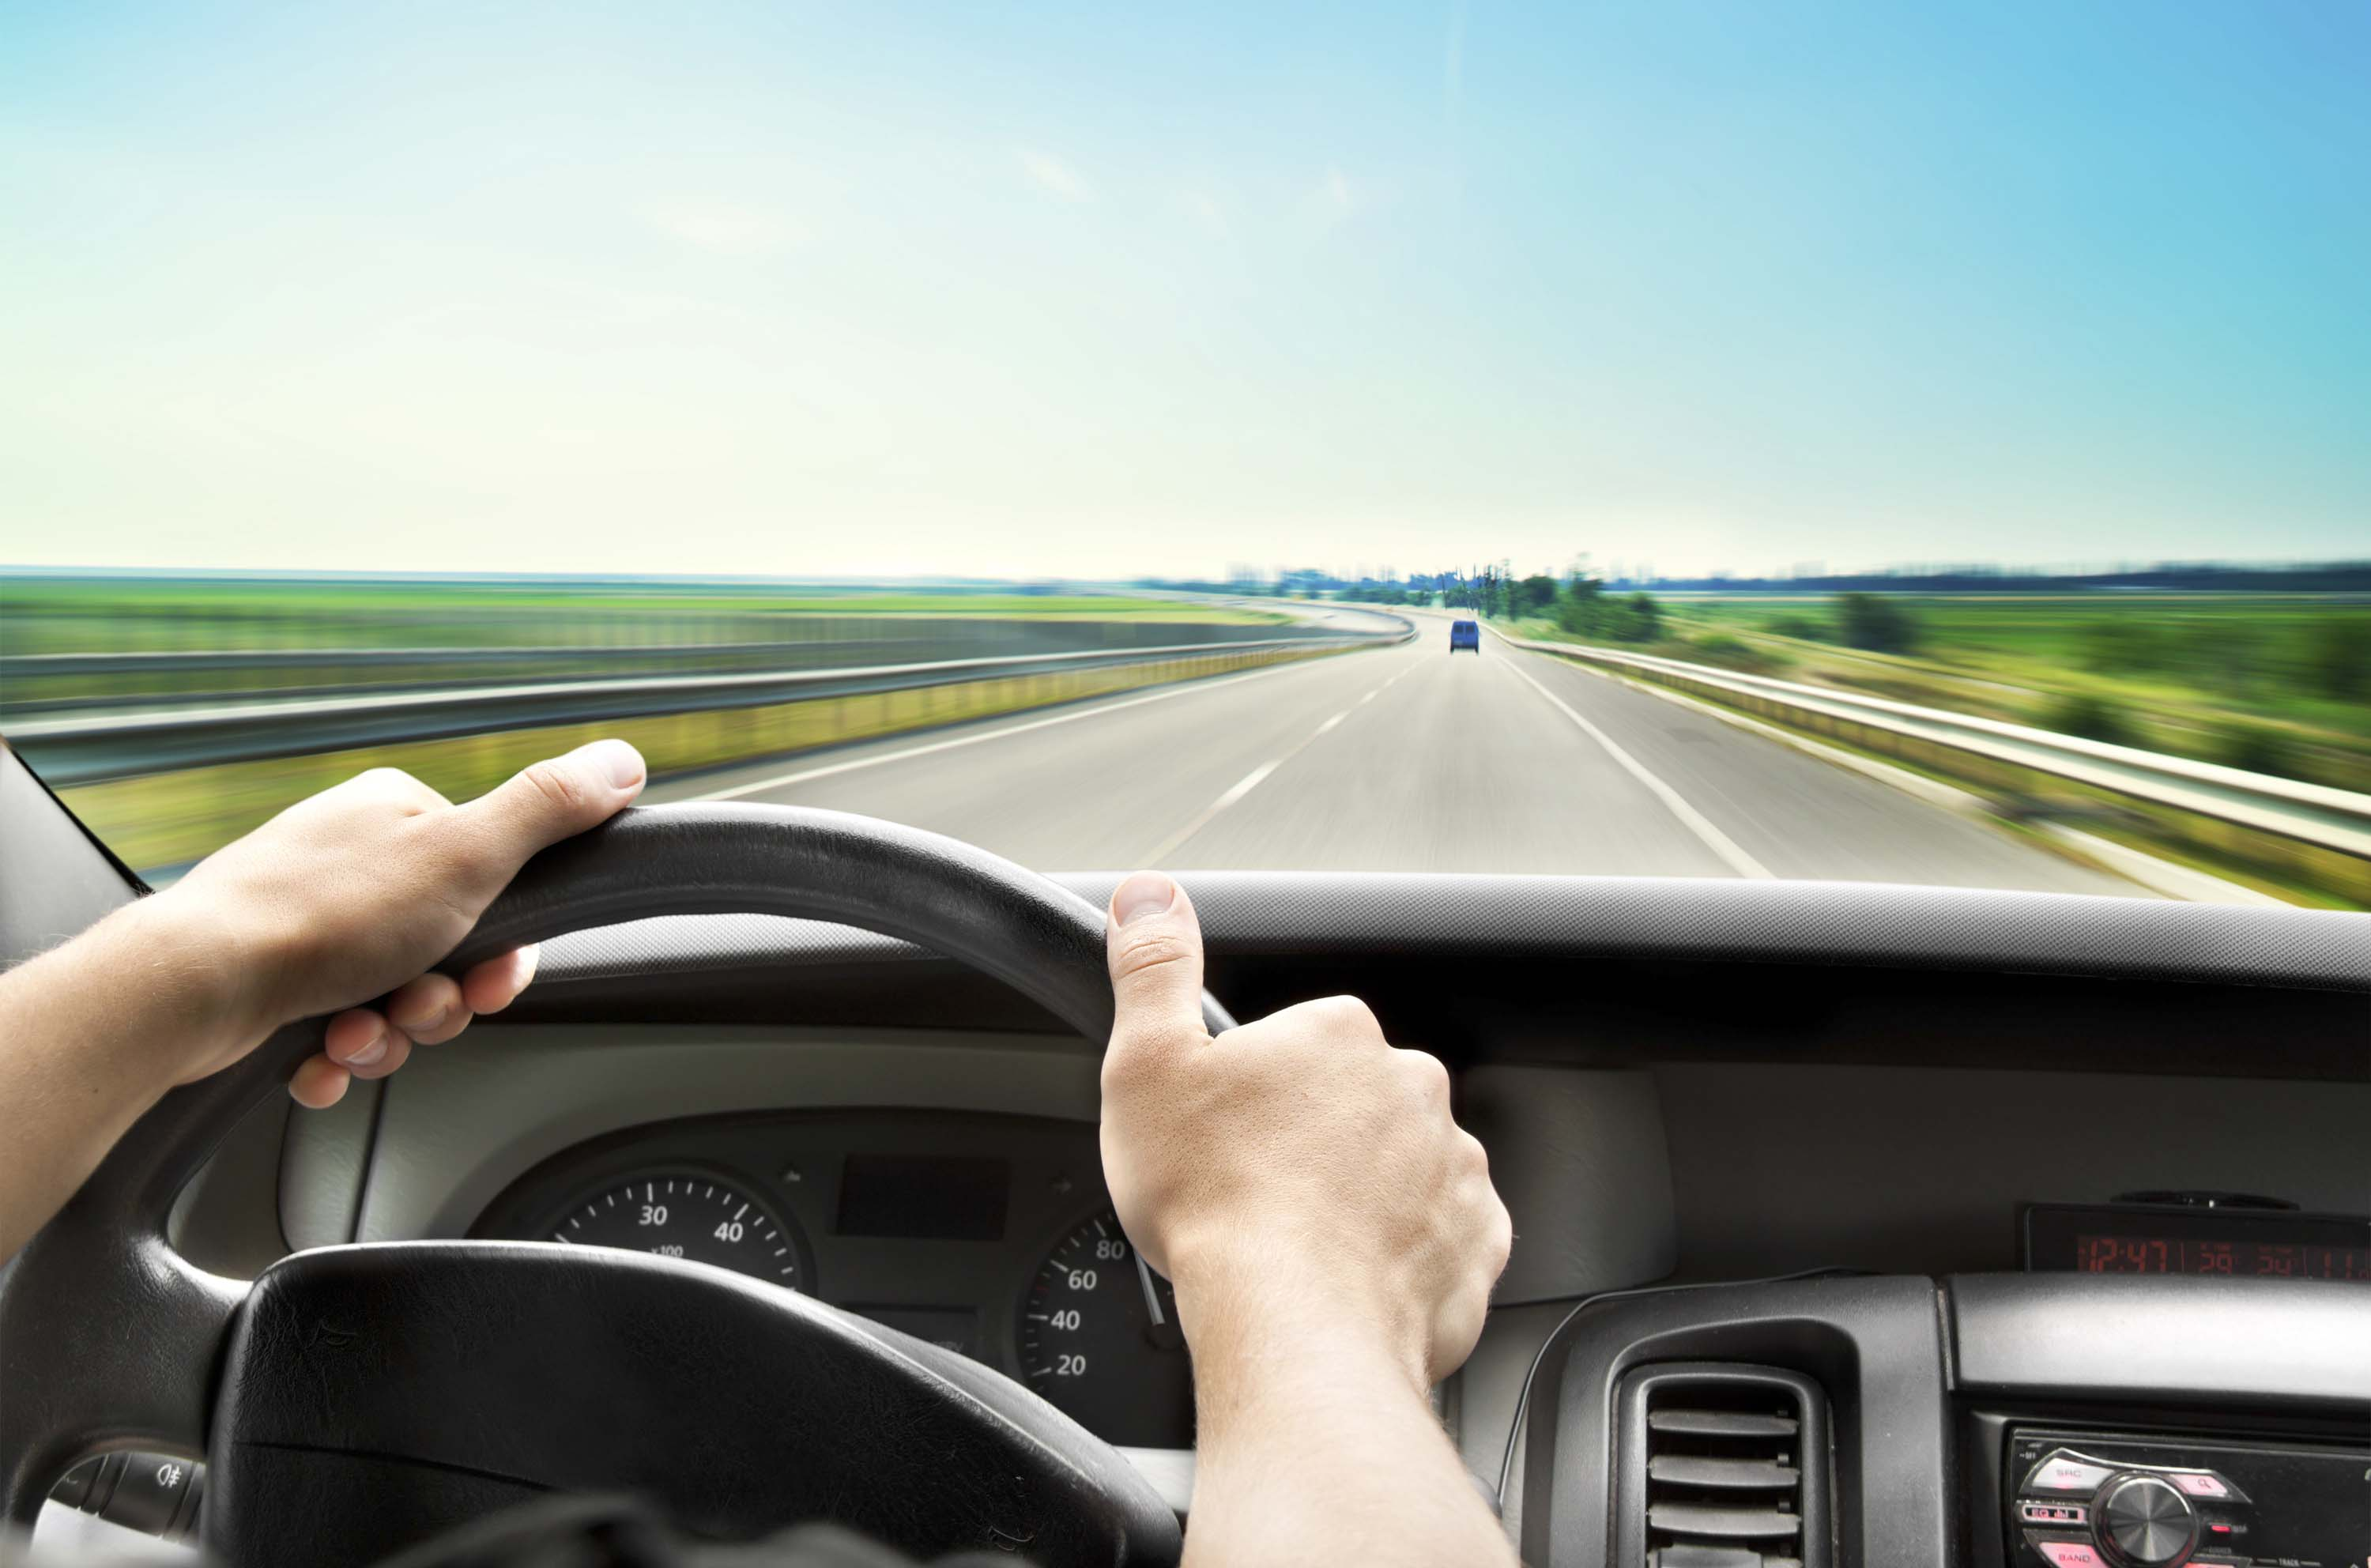
\includegraphics[width=\linewidth,height=0.7\textheight,keepaspectratio]{images/driving.jpg}
		\caption{Driving}
		\label{fig_driving}
		\credit{http://combiboilersleeds.com/keywords/driving-1.html}
	\end{figure}	
\end{frame}
\begin{frame}{Example}
	\begin{figure}
		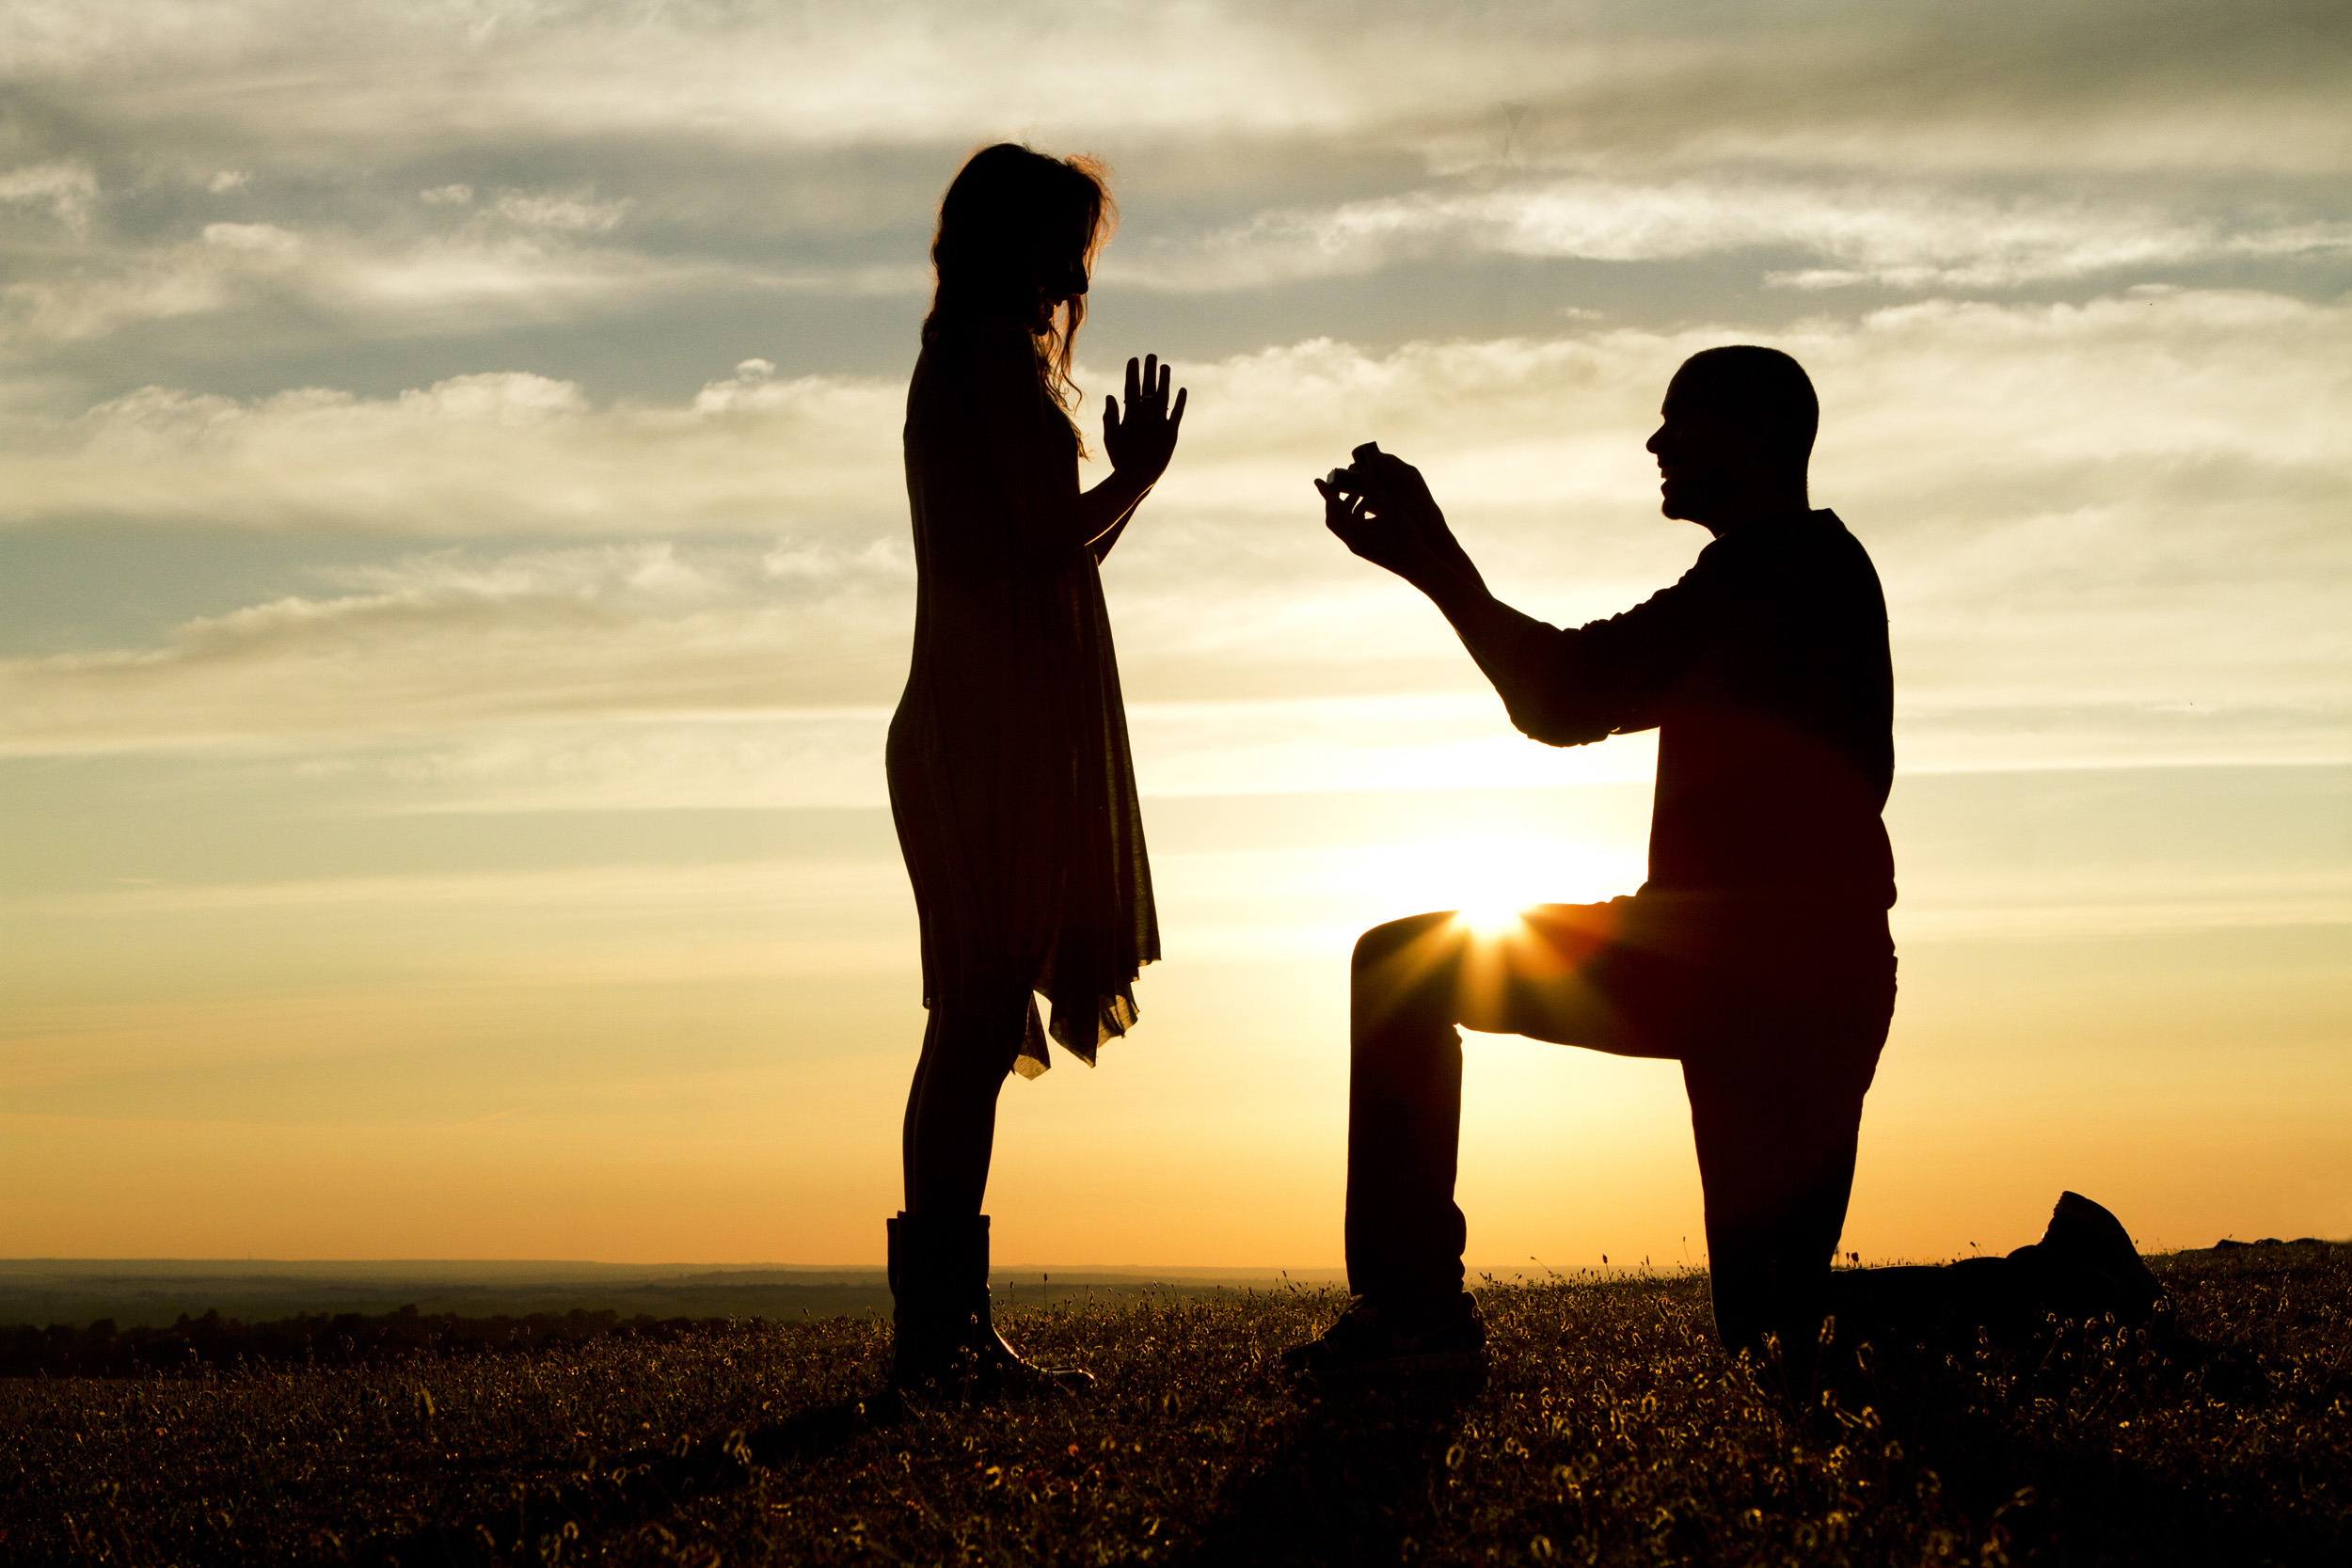
\includegraphics[width=\linewidth,height=0.7\textheight,keepaspectratio]{images/proposal.jpg}
		\caption{Deciding whom to marry}
		\credit{http://engaged.robbinsbrothers.com/wp-content/uploads/2014/01/propose-live-on-tv.jpeg?7f685f}
	\end{figure}	
\end{frame}
\begin{frame}{Example}
	\begin{figure}
		
\includegraphics[width=\linewidth,height=0.4\textheight,keepaspectratio]{images/thinker.png}
		\credit{https://cdn.shopify.com/s/files/1/1061/1924/files/Thinking_Face_Emoji.png?9898922749706957214}
	\end{figure}
	\begin{block}{}
		"That doesn't look right. Can we check the calculations again?"
	\end{block}	
\end{frame}
%--------------------------------------------------------------------------------------------
\subsection{How is intuition helpful?}
%--------------------------------------------------------------------------------------------
\begin{frame}{Deal with complexity}
	\begin{columns}[T]
		\begin{column}{.5\textwidth}
			\begin{itemize}{}
				 \item{Instinctively understand what information is unimportant \parencite{gert}}
			\end{itemize}
		\end{column}
		\begin{column}{.5\textwidth}
			\begin{figure}
				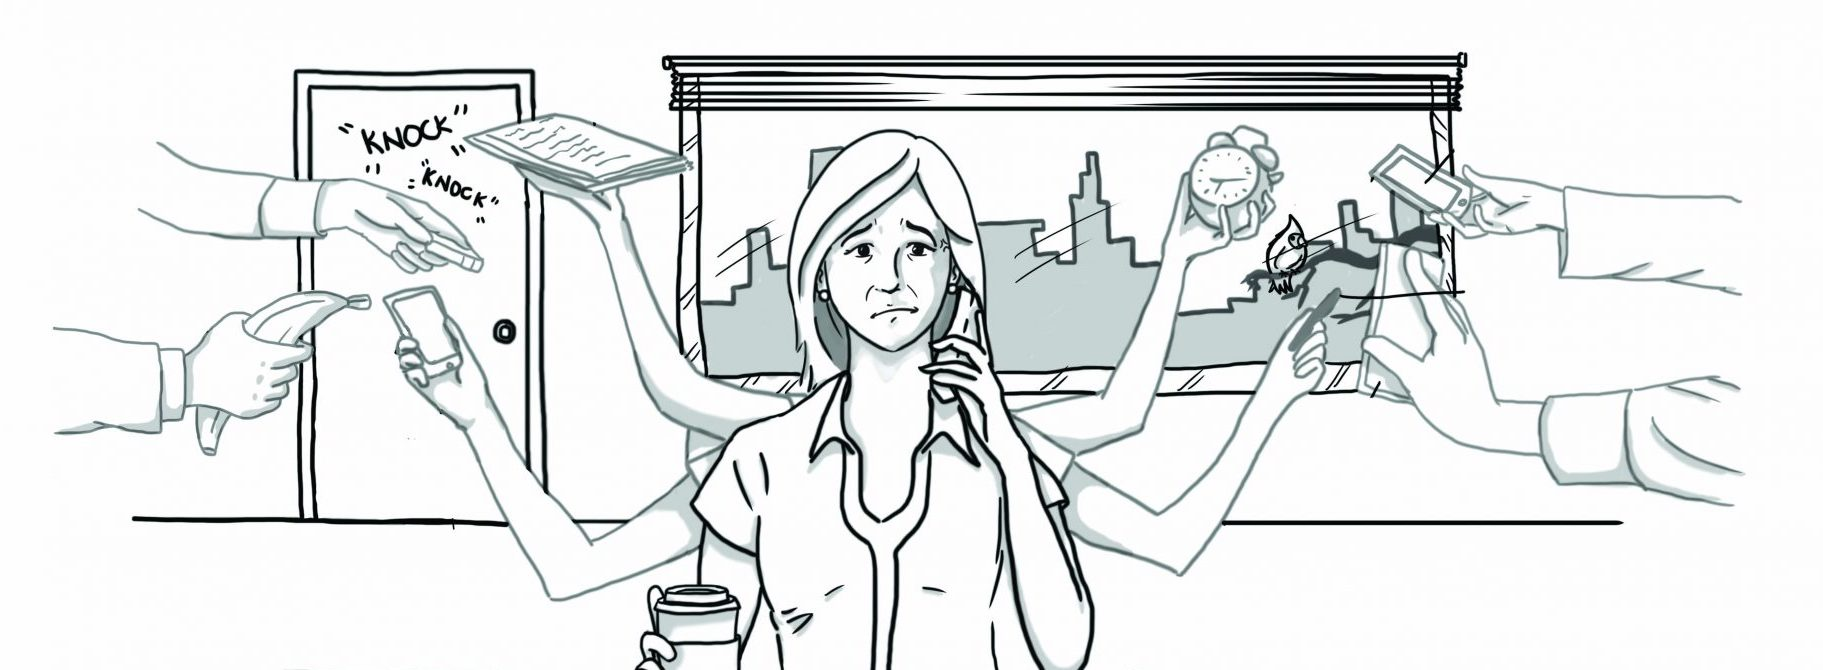
\includegraphics[width=\linewidth,height=0.7\textheight,keepaspectratio]{images/information.jpg}
				\caption{Machines can't do what we can, at least not yet!}
				\credit{http://thebrieflab.com/wp-content/uploads/2016/12/Information_overload-e1481756393396.jpeg}
			\end{figure}
		\end{column}
	\end{columns}
\end{frame}
\begin{frame}{High quality decisions in very little time}
	\begin{columns}[T]
		\begin{column}{.5\textwidth}
			\begin{block}{}
						"From a managerial perspective, the speed of
						intuiting is not only taken for granted but is
						often seen as a primary motivator for developing
						and employing intuition at work \parencite{intuition}."
			\end{block}
		\end{column}
		\begin{column}{.5\textwidth}
			\begin{figure}
				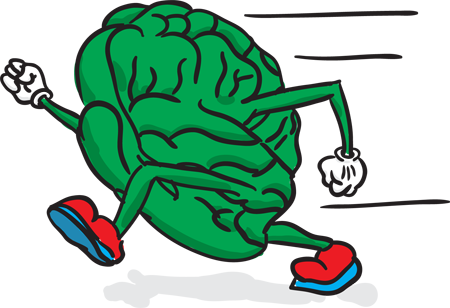
\includegraphics[width=\linewidth,height=0.7\textheight,keepaspectratio]{images/brain.png}
				\caption{Intuition is fast!}
				\credit{http://mea.com.au/upload/Blog/Brain_Faster.png}
			\end{figure}
		\end{column}
	\end{columns}
\end{frame}
\begin{frame}{Continued career progression}
	\begin{columns}[T]
		\begin{column}{.5\textwidth}
			\begin{block}{}
				"The effective use of intuition has even been seen as critical in differentiating successful top executives and board members from lower-level managers and dysfunctional boards \parencite{intuition}."
			\end{block}
		\end{column}
		\begin{column}{.5\textwidth}
			\begin{figure}
				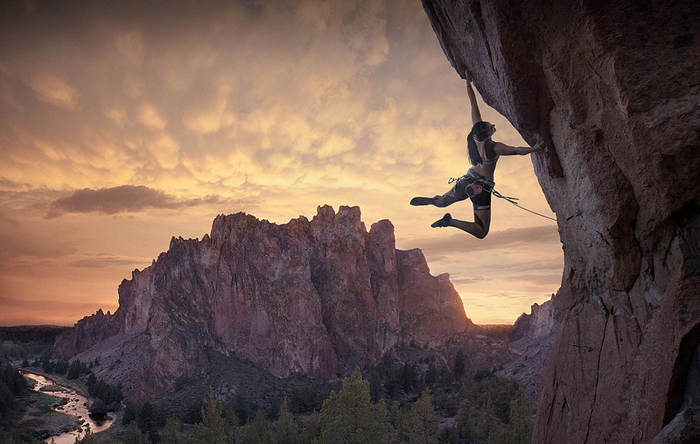
\includegraphics[width=\linewidth,height=0.7\textheight,keepaspectratio]{images/climber.jpg}
				\caption{For a climber intuition is a necessity}
				\credit{https://d36tnp772eyphs.cloudfront.net/blogs/1/2014/08/Smith-Rock-940x595.jpg}
			\end{figure}
		\end{column}
	\end{columns}
\end{frame}
\begin{frame}{Intuitive tools cost less time in the long run}
	\begin{columns}[T]
		\begin{column}{.5\textwidth}
			\begin{itemize}
				\item Tools that employees use repeatedly
					\begin{itemize}
							\item Organisational structures
							\item Processes
							\item User guides
							\item Websites
							\item Computer programs [off the shelf and in-house]
							\item Data
							\item Machinery
					\end{itemize}
				\item Reduced training costs,  times
				\item More effective training
				\item Reduced tool usage times
			\end{itemize}
		\end{column}
		\begin{column}{.5\textwidth}
			\begin{figure}
				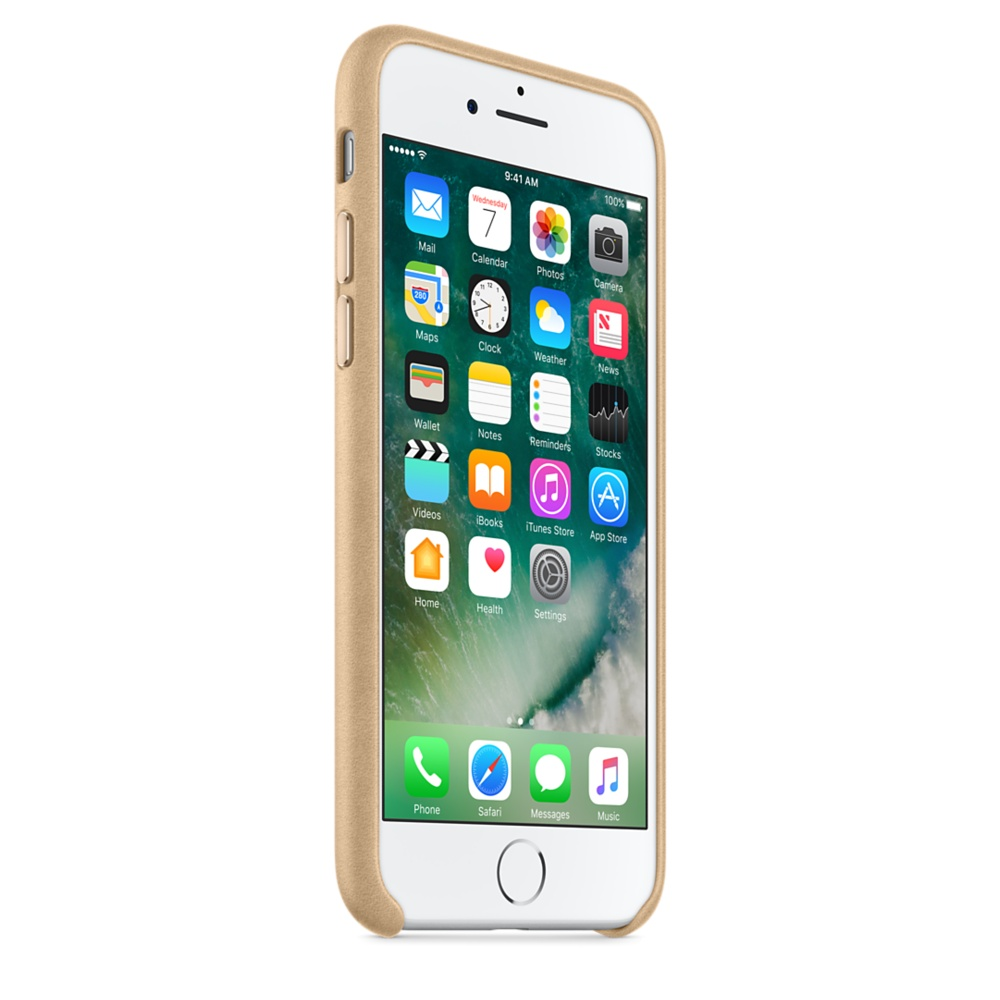
\includegraphics[width=\linewidth,height=0.5\textheight,keepaspectratio]{images/iphone.jpg}
				\caption{Intuitive designs are "understandable without the use of instructions" \parencite{design}}
			\end{figure}
		\end{column}
	\end{columns}
\end{frame}

%--------------------------------------------------------------------------------------------
\subsection{Why is intuition particularly relevant today?}
%--------------------------------------------------------------------------------------------
\begin{frame}{Our work is getting more and more complex}
	\begin{figure}
		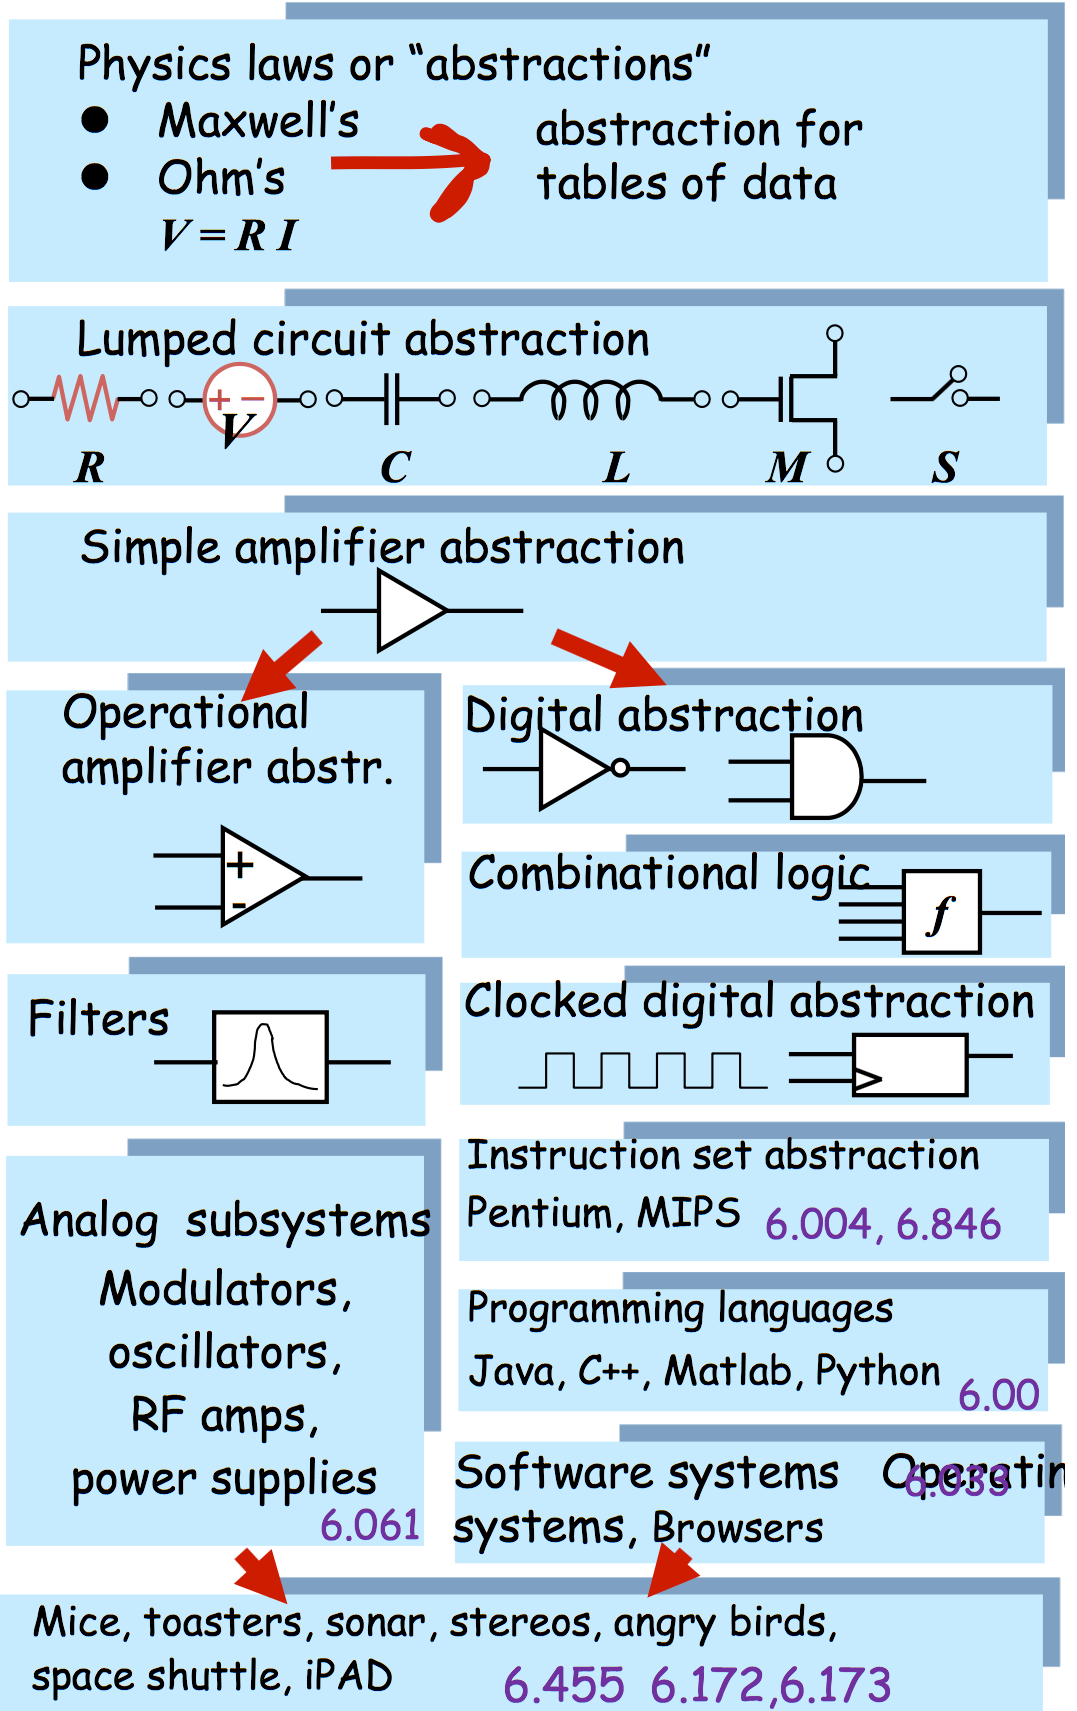
\includegraphics[width=\linewidth,height=0.78\textheight,keepaspectratio]{images/lumped.png}
		\caption{Lumped abstraction \parencite{lumped}}
		\label{fig_lumped}
	\end{figure}
\end{frame}
\begin{frame}{Rapidly changing environements}
	\begin{columns}[T]
		\begin{column}{.5\textwidth}
			\begin{itemize}
				\item The business environment is changing more rapidly than ever before
				\item Intuition helps us focus on what is important, and to seize opportunities
			\end{itemize}
		\end{column}
		\begin{column}{.5\textwidth}
			\begin{figure}
				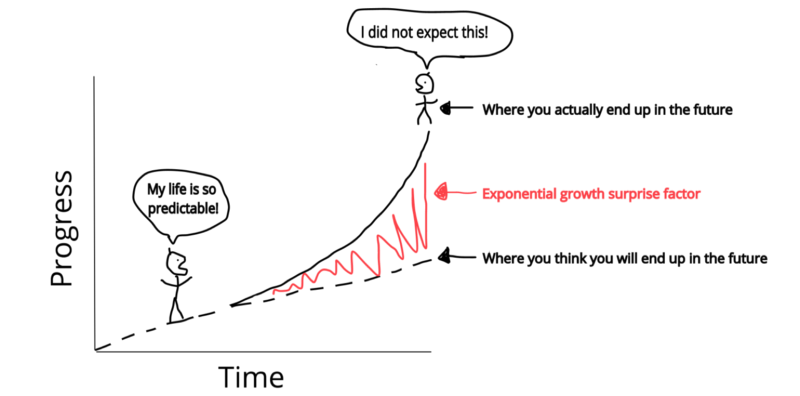
\includegraphics[width=\linewidth,height=0.7\textheight,keepaspectratio]{images/exponential.png}
				\caption{Exponential growth}
				\credit{http://roadmap2retire.com/2016/06/disruptive-technologies-exponential-growth/}
			\end{figure}
		\end{column}
	\end{columns}
\end{frame}
\begin{frame}{People are staying in the same job for less time!}
	\begin{columns}[T]
		\begin{column}{.5\textwidth}
			\begin{itemize}
				\item Job-hopping is on the rise
				\item Less time to develop intuition
				\item Potential loss of expertise
			\end{itemize}
		\end{column}
		\begin{column}{.5\textwidth}
			\begin{figure}
				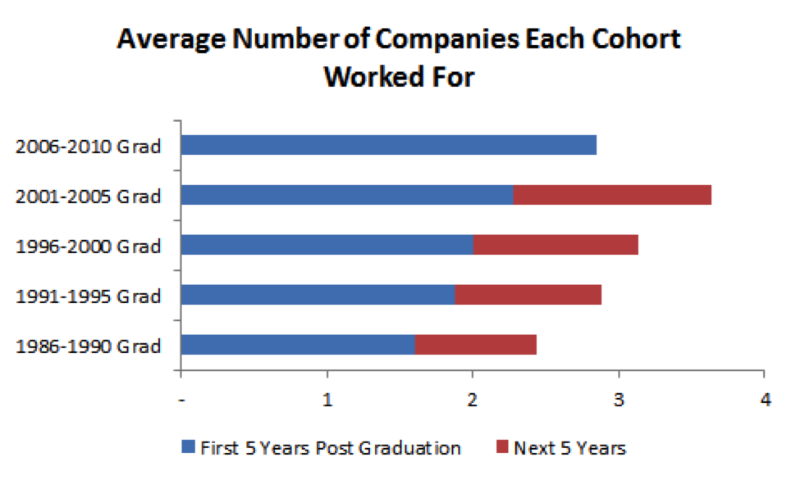
\includegraphics[width=\linewidth,height=0.7\textheight,keepaspectratio]{images/jobhop.png}
				\caption{Job-hopping is on the rise \parencite{berger}}
			\end{figure}
		\end{column}
	\end{columns}
\end{frame}

%=====================================================================
\section{How could we mould a highly intuitive workforce?}
%--------------------------------------------------------------------------------------------
%--------------------------------------------------------------------------------------------
\subsection{Natural factors in developing intuition}
%--------------------------------------------------------------------------------------------
\begin{frame}{Natural factors in developing intuition}
	\begin{figure}
		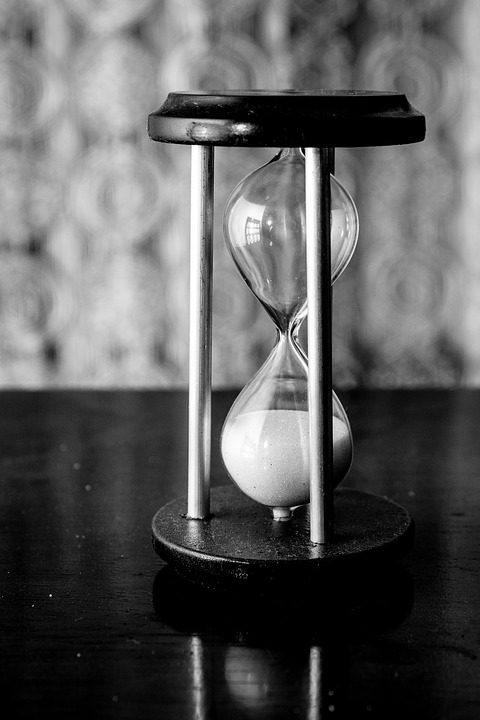
\includegraphics[width=\linewidth,height=0.6\textheight,keepaspectratio]{images/hourglass.jpg}
		\caption{Intuition comes naturally with time, repetition and experience, but time is a finite resource}
		\credit{https://encrypted-tbn3.gstatic.com/images?q=tbn:ANd9GcTNOtj0C1cEART16GSmhoPrnpYlWfK2rY6sPyUrgJBBv6v1KNb2ag}
		\label{fig_time}
	\end{figure}
\end{frame}
\subsection{Promoting intuition in the workplace}
\begin{frame}{Hold on to our employees - Retention rates}
	\begin{columns}[T]
		\begin{column}{.5\textwidth}
			\begin{itemize}
				\item Show an appreciation
				\item Provide exposure to a lot of opportunities
				\item Offer training and development
				\item Encourage job changes between related disciplines
				\item ... this topic is worth a presentation on its own right
			\end{itemize}
		\end{column}
		\begin{column}{.5\textwidth}
			\begin{figure}
				
\includegraphics[width=\linewidth,height=0.5\textheight,keepaspectratio]{images/lovemyjob.jpg}
				\caption{A good salary isn't enough to keep good employees.}
				\credit{https://t4.ftcdn.net/jpg/00/68/46/57/240_F_68465752_GLciUylvckK6mZFwwR95XGTETACcgCOm.jpg}
			\end{figure}
		\end{column}
	\end{columns}
\end{frame}
\begin{frame}{Invest in intuitive tools}
	\begin{columns}[T]
		\begin{column}{.5\textwidth}
			\begin{itemize}
				\item Invest upfront in developing really good, intuitive User Interfaces [UI]				\item This would require training people to create good UIs
				\item People are generally bad at designing tools for themselves or their teams!
				\item \textbf{The lifecycle costs of using those tools will be much less as a result}
			\end{itemize}
		\end{column}
		\begin{column}{.5\textwidth}
			\begin{figure}
				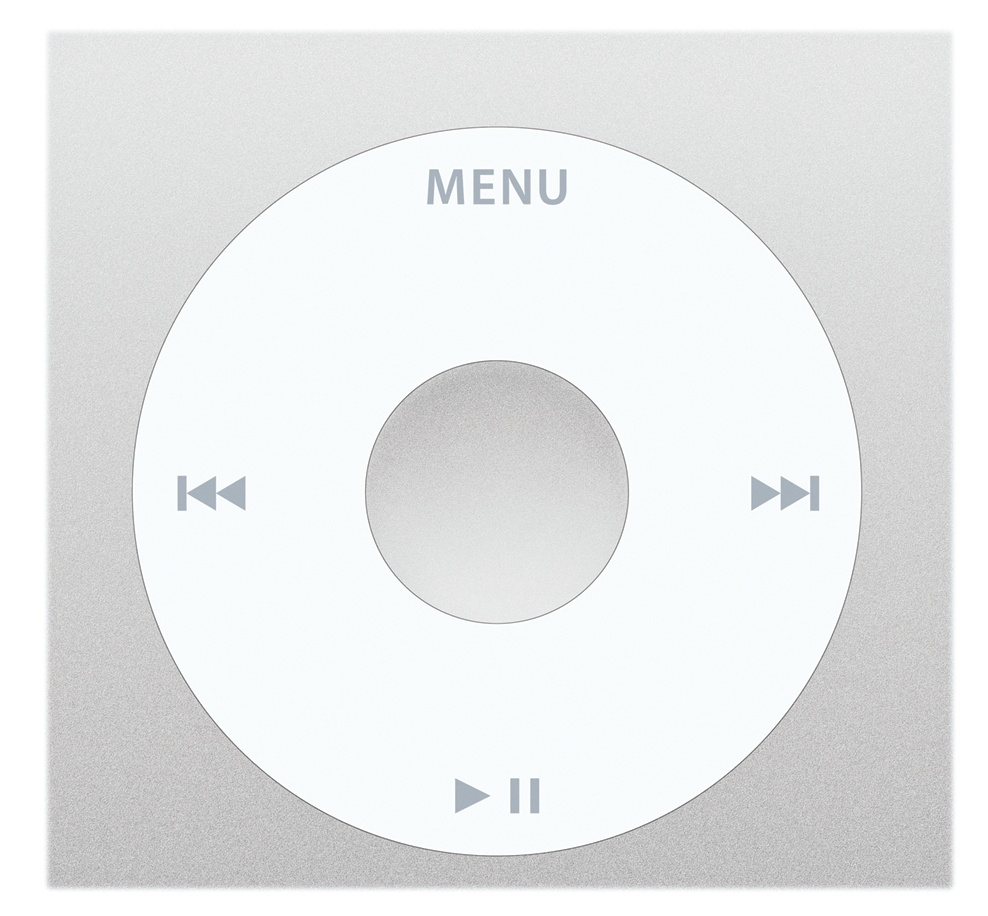
\includegraphics[width=\linewidth,height=0.5\textheight,keepaspectratio]{images/ipodwheel.jpg}
				\caption{The iPod click wheel}
				\credit{https://www.safaribooksonline.com/library/view/ipod-the-missing/9780596155834/httpatomoreillycomsourceoreillyimages216198.png.jpg}
			\end{figure}
		\end{column}
	\end{columns}
\end{frame}
\begin{frame}{Explicit training - Active}
	\begin{columns}[T]
		\begin{column}{.5\textwidth}
			\begin{itemize}
				\item Analogy
				\item Online lectures
				\item Static images
				\item Animations
				\item Interactive animations
				\item Augmented reality
				\item Virtual reality
			\end{itemize}
		\end{column}
		\begin{column}{.5\textwidth}
			\begin{figure}
				\includegraphics<1>[width=\linewidth,height=0.5\textheight,keepaspectratio]{images/massSpring.png}
				\includegraphics<2>[width=\linewidth,height=0.5\textheight,keepaspectratio]{images/teaching.jpg}
				\caption{
					\only<1>{The famous mass-spring analogy}
					\only<2>{Teaching style has a significant impact}}
			\only<1>{\credit{https://ugc.futurelearn.com/uploads/images/9d/75/hero_9d756280-d14c-43ed-b035-aec3e4b4d4a7.png}}
			\only<2>{\credit{http://c1.thejournal.ie/media/2013/06/maths-equation-one-million-dollars-390x285.jpg}}
			\end{figure}
		\end{column}
	\end{columns}
\end{frame}
\begin{frame}{Implicit training - On the job, natural}
	\begin{columns}[T]
		\begin{column}{.5\textwidth}
			\begin{itemize}
				\item You can try, but you just can't replace an experienced person with  documentation
				\item Mix experts and novices and encourage collaboration
				\item Repetition
				\item Encourage asking questions
				\item Encourage asking for help
				\item Provide feedback
			\end{itemize}
		\end{column}
		\begin{column}{.5\textwidth}
			\begin{figure}
				\includegraphics<1,2>[width=\linewidth,height=0.5\textheight,keepaspectratio]{images/expertsandnovices.jpg}
				\includegraphics<3>[width=\linewidth,height=0.5\textheight,keepaspectratio]{images/repetition.jpg}
				\caption{
					\only<1,2>{Experts and novices can learn from each other}
				    \only<3>{Repetition}}
			    \only<1,2>{\credit{http://www.gannett-cdn.com/-mm-/6c97cde1d27e994806d61fc6f7a2d6724ac53087/c=0-139-4331-2573&r=x1803&c=3200x1800/local/-/media/USATODAY/USATODAY/2014/08/22/1408736863000-boss.jpg}}
			    \only<3>{\credit{http://learnenglishteens.britishcouncil.org/sites/teens/files/field/image/istock_000016212764small1.jpg}}
			\end{figure}
		\end{column}
	\end{columns}
\end{frame}

%=====================================================================
\section{Conclusion}
\begin{frame}
\begin{block}{Albert Einstein}
	“The intuitive mind is a sacred gift and the rational mind is a faithful servant.We have created a society that honors the servant and has forgotten the gift.”
\end{block}
\begin{itemize}
	\item{Intuition is \textbf{important}}
	\item{Intuition is particularly relevant \textbf{today}}
	\item{We can \textbf{promote} intuition. We just need to make the effort!}
	\item{The future is looking good! I am excited! Aren't you?}
\end{itemize}
\end{frame}
\begin{frame}[allowframebreaks]
	\frametitle{References}
	\printbibliography[heading=none]
\end{frame}
\end{document}